\documentclass{jhwhw}

\title{Tutorial A2\\Numerical Methods of Finding Roots}
\author{Eytan Chong}
\date{2024-02-29}

\begin{document}
    \problem{}
        Without using a graphing calculator, show that the equation $x^3+2x^2-2=0$ has exactly one positive root.

        This root is denoted by $\alpha$ and is to be found using two different iterative methods, starting with the same initial approximation in each case.

        \begin{enumerate}
            \item Show that $\alpha$ is a root of the equation $x = \sqrt{\dfrac2{x+2}}$, and use the iterative formula $x_{n+1} = \sqrt{\dfrac2{x_n + 2}}$, with $x_1 = 1$, to find $\alpha$ correct to 2 significant figures.
            \item Use the Newton-Raphson method, with $x_1=1$, to find $\alpha$ correct to 3 significant figures.
        \end{enumerate}

    \solution
        Let $f(x) = x^3 + 2x^2 - 2 =0$. Consider $f^\prime(x) = 3x^2 + 4x$. Observe that for all $x > 0$, we have $f^\prime(x) > 0$. Hence, $f(x)$ is increasing for all positive $x$. Note that $f(0) = -2 < 0$ and $f(1) = 1 > 0$. Thus, $f(x)$ has exactly one positive root.
        
        \part
            We know $f(\alpha) = 0$. Hence,

            \begin{alignat*}{2}
                &&\alpha^3 + 2\alpha^2 - 2 &= 0 \\
                \implies&& \alpha^2 (\alpha + 2) &= 2 \\
                \implies&& \alpha^2 &= \dfrac2{\alpha + 2} \\
                \implies&& \alpha &= \sqrt{\dfrac2{\alpha + 2}} \reject{$\alpha = -\sqrt{\dfrac2{\alpha + 2}} \because \alpha > 0$} 
            \end{alignat*}

            Thus, $\alpha$ is a root of the equation $x = \sqrt{\dfrac2{x+2}}$.

            \begin{alignat*}{2}
                && x_1 &= 1 \\
                \implies&&x_2 &= \sqrt{\dfrac2{x_1 + 2}} = 0.81650 \\
                \implies&&x_3 &= \sqrt{\dfrac2{x_2 + 2}} = 0.84268 \\
                \implies&&x_4 &= \sqrt{\dfrac2{x_3 + 2}} = 0.83879
            \end{alignat*}

            \boxt{
                $\alpha = 0.84 \tosf2$
            }

        \part
            \begin{alignat*}{2}
                && x_1 &= 1 \\
                \implies&&x_2 &= \nrm{x_1}{f} = 0.857143 \\
                \implies&&x_3 &= \nrm{x_2}{f} = 0.839545 \\
                \implies&&x_4 &= \nrm{x_3}{f} = 0.839287 \\
                \implies&&x_5 &= \nrm{x_4}{f} = 0.839287
            \end{alignat*}

            \boxt{
                $\alpha = 0.839 \tosf3$
            }

    \problem{}
        \begin{enumerate}
            \item Show that the tangent at the point $(e, 1)$ to the graph $y=\ln x$ passes through the origin, and deduce that the line $y=mx$ cuts the graph $y=\ln x$ in two points provided that $0 < m <  \dfrac1e$.
            \item For each root of the equation $\ln x = \dfrac13 x$, find an integer $n$ such that the interval $n < x < n+1$ contains the root. Using linear interpolation, based on $x=n$ and $x = n+1$, find a first approximation to the smaller root, giving your answer to 1 decimal place. Using your first approximation, obtain, by the Newton-Raphson method, a second approximation to the smaller root, giving your answer to 2 decimal plces.
        \end{enumerate}

    \solution
        \part
            Using the point slope formula, we see that the equation of the tangent at the point $(e,1)$ is given by

            \begin{alignat*}{2}
                &&y - 1 &= \left. \der{y}{x}\right|_{x=e} (x - e) \\
                \implies && y &= \left. \dfrac1x \right|_{x=e}(x-e) + 1 \\
                \implies && y &= \dfrac1e (x-e) + 1 \\
                \implies && y &= \dfrac1e x
            \end{alignat*}

            Since $x=0$, $y=0$ is clearly a solution, the tangent at the point $(e,1)$ passes through the origin.

            From the graph below, it is clear that for $y = mx$ to intersect $y = \ln x$ twice, we must have $0 < m < \dfrac1e$.

            \begin{center}
                \begin{tikzpicture}[trim axis left, trim axis right]
                    \begin{axis}[
                        domain = -1:5,
                        samples = 50,
                        axis y line=middle,
                        axis x line=middle,
                        xtick = {1},
                        ytick = \empty,
                        ymin=-0.5,
                        xlabel = {$x$},
                        ylabel = {$y$},
                        legend cell align={left},
                        legend pos=outer north east,
                        after end axis/.code={
                            \path (axis cs:0,0) 
                                node [anchor=south east] {$O$};
                            }
                        ]
                        \addplot[red!50] {ln(x)};

                        \addlegendentry{$y=\ln x$};

                        \addplot[blue!50] {1/e * x};

                        \addlegendentry{$y=\frac1e x$};

                        \fill (axis cs: 2.718, 1) circle[radius=2.5pt] node[anchor=south east] {$(e, 1)$};
                    \end{axis}
                \end{tikzpicture}
            \end{center}
            
        \part
            Consider $f(x) = \dfrac13 x - \ln x$. Let $\alpha$ be the smaller root to $f(x) = 0$.
            
            Observe that $f(1) = 1 > 0$ and $f(2) = -0.03 < 0$. Thus, for the smaller root $\alpha$, $n = 1$.

            \boxt{
                Smaller root: $n = 1$
            }

            Observe that $f(4) = -0.05 < 0$ and $f(5) = 0.06 > 0$. Hence, for the larger root $\beta$, $n = 4$.

            \boxt{
                Larger root: $n = 4$
            }

            Using linear interpolation, we have that $\alpha$ is approximately equal to $x_1$, where

            \begin{equation*}
                \begin{aligned}
                    x_1 &= \dfrac{1f(2) - 2f(1)}{f(2) - f(1)} \\
                    &= 1.9 \todp{1}
                \end{aligned}
            \end{equation*}

            \boxt{
                First approximation = 1.9
            }

            Using the Newton-Raphson method, 

            \begin{alignat*}{2}
                && x_1 &= 1.9 \\
                \implies&&x_2 &= \nrm{x_1}{f} = 1.85585 \\
                \implies&&x_3 &= \nrm{x_2}{f} = 1.85718
            \end{alignat*}

            \boxt{
                $\alpha = 1.86 \todp{2}$
            }

    \problem{}
        Find the exact coordinates of the turning points on the graph of $y = f(x)$ where $f(x) = x^3-x^2-x-1$. Deduce that the equation $f(x) = 0$ has only one real root $\alpha$, and prove that $\alpha$ lies between 1 and 2. Use the Newton-Raphson method applied to the equation $f(x) = 0$ to find a second approximation $x_2$ to $\alpha$, taking $x_1$, the first approximation, to be 2. With reference to a graph of $y=f(x)$, explain why all further approximations to $\alpha$ by this process are always larger than $\alpha$.

    \solution
        For turning points, $f^\prime(x) = 0$.

        \begin{alignat*}{2}
            &&f^\prime(x) &= 0 \\
            \implies&& 3x^2-2x-1 &= 0\\
            \implies&& (3x+1)(x-1) &= 0
        \end{alignat*}

        Hence, $x = -\dfrac13$ or $x = 1$. When $x = -\dfrac13$, we have $y = -0.815$, giving the coordinate $(-\dfrac13, -0.815)$. When $x = 1$, we have $y = -2$, giving the coordinate $(1, -2)$.

        \boxt{
            The coordinates of the turning points are $(-\dfrac13, -0.815)$ and $(1,-2)$.
        }

        Observe that $f(x)$ is strictly increasing for all $x > 1$. Since $f(1) = -2 < 0$ and $f(2) = 1 > 0$, the equation $f(x) = 0$ has only one real root.

        Using the Newton-Raphson method with $x_1 = 2$, we have $x_2 = \nrm{x_1}{f} = \dfrac{13}7$.

        \boxt{
            $x_2 = \dfrac{13}7$
        }

        \begin{center}
            \begin{tikzpicture}[trim axis left, trim axis right]
                \begin{axis}[
                    domain = 1.5:2.5,
                    samples = 50,
                    axis y line=middle,
                    axis x line=middle,
                    xtick = {1.8393, 1.994, 2.4},
                    xticklabels = {$\alpha$, $x_2$, 2},
                    ytick = \empty,
                    xlabel = {$x$},
                    ylabel = {$y$},
                    ymin = -2,
                    legend cell align={left},
                    legend pos=outer north east,
                    after end axis/.code={
                        \path (axis cs:1.5,0) 
                            node [anchor=east] {$O$};
                        }
                    ]

                    \draw[thick,black!70,TwoMarks=0.1] (1.5,0) -- (1.8,0);

                    \addplot[red!50] {x^3-x^2-x-1};

                    \addlegendentry{$y=x^3-x^2-x-1$};

                    \draw[dotted, very thick] (2.4, 0) -- (2.4, 4.644);

                    \addplot[dotted, very thick] {11.48 * (x-2.4) + 4.644};

                \end{axis}
            \end{tikzpicture}
        \end{center}

        Since $x_2$ lies on the right of $\alpha$, the Newton-Raphson method gives an over-estimation given an initial approximation of 2. Thus, all further approximations to $\alpha$ will also be larger than $\alpha$.

    \problem{}
        A curve $C$ has equation $y = x^5 + 50x$. Find the least value of $\der{y}{x}$ and hence give a reason why the equation $x^5+50x=10^5$ has exactly one real root. Use the Newton-Raphson method, with a suitable first approximation, to find, correct to 4 decimal places, the root of the equation $x^5+50x=10^5$. You should demonstrate that your answer has the required accuracy.

    \solution
        Since $y = x^5 + 50x$, we know that $\der{y}{x} = 5x^4 + 50$. Since $x^4 \geq 0$ for all real $x$, the minimum value of $\der{y}{x}$ is 50.

        \boxt{
            $\min \der{y}{x} = 50$
        }

        Let $f(x) = x^5 + 50x$. Since $\min \der{f}{x} = 50 > 0$, we have that $f(x)$ is a strictly increasing function. Thus, $f(x)$ will intersect only once with the line $y = 10^5$. Hence, the equation $x^5 + 50x = 10^5$ has exactly one real root.

        Observe that $f(9) = -40901 < 0$ and $f(10) = 50 > 0$. Thus, there must be a root on the interval $(9, 10)$. We now use the Newton-Raphson method with $x_1 = 9$ as the first approximation.

        \begin{alignat*}{2}
            && x_1 &= 9 \\
            \implies&&x_2 &= \nrm{x_1}{f} = 10.2178921 \\
            \implies&&x_3 &= \nrm{x_2}{f} = 10.0017491 \\
            \implies&&x_4 &= \nrm{x_3}{f} = 9.9901221 \\
            \implies&&x_5 &= \nrm{x_4}{f} = 9.9899912 \\
            \implies&&x_6 &= \nrm{x_5}{f} = 9.9899900 
        \end{alignat*}

        \boxt{
            The root is $9.9900 \todp{4}$.
        }

        Observe that $f(9.98995) = -2.00 < 0$ and $f(9.99005) = 3.00 > 0$. Hence, the root lies in the interval $(9.98995, 9.99005)$. Thus, the calculated root has the required accuracy.

    \problem{}
        \begin{enumerate}
            \item A function $f$ is such that $f(4) = 1.158$ and $f(5) = -3.381$, correct to 3 decimal places in each case. Assuming that there is a value of $x$ between 4 and 5 for which $f(x) = 0$, use linear interpolation to estimate this value.
            
            For the case when $f(x) = \tan x$, and $x$ is measured in radians, the value of $f(4)$ and $f(5)$ are as given above. Explain, with the aid of a sketch, why linear interpolation using these values does not give an approximation to a solution of the equation $\tan x = 0$.

            \item Show, by means of a graphical argument or otherwise, that the equation $\ln (x-1) = -2x$ has exactly one real root, and show that this root lies between 1 and 2. 
            
            The equation may be written in the form $\ln (x-1) + 2x = 0$. Show that neither $x=1$ nor $x=2$ is a suitable initial value for the Newton-Rapson method in this case.

            The equation may also be written in the form $x - 1 - e^{-2x} = 0$. For this form, use two applications of the Newton-Raphson method, starting with $x=1$, to obtain an approximation to the root, giving 3 decimal places in your answer.
        \end{enumerate}

    \solution
        \part
            Let the root of $f(x) = 0$ be $\alpha$. Using linear interpolation on the interval $[4, 5]$, we have

            \begin{equation*}
                \begin{aligned}
                    \alpha &= \dfrac{4f(5) - 5f(4)}{f(5) - f(4)} \\
                    &= 4.255 \todp{3} 
                \end{aligned}
            \end{equation*}

            \boxt{
                $\alpha = 4.255 \todp3$
            }

            \begin{center}
                \begin{tikzpicture}[trim axis left, trim axis right]
                    \begin{axis}[
                        samples = 500,
                        axis y line=middle,
                        axis x line=middle,
                        xtick = {4, 5},
                        ytick = \empty,
                        xlabel = {$x$},
                        ylabel = {$y$},
                        xmin=3,xmax=6,ymin=-10,ymax=10,
                        legend cell align={left},
                        legend pos=outer north east,
                        after end axis/.code={
                            \path (axis cs:3,0) 
                                node [anchor=east] {$O$};
                            }
                        ]

                        \draw[thick,black!70,TwoMarks=0.1] (pi, 0) -- (pi + 0.3,0);

                        \addplot[red!50, domain=pi:3*pi/2-0.01] {tan(\x r)};

                        \addplot[red!50, domain=3*pi/2+0.01:5*pi/2-0.01] {tan(\x r)};

                        \draw[dotted, very thick] (axis cs:3*pi/2, -10) -- (axis cs:3*pi/2, 10);
                        \node[anchor=north west] at (axis cs:3*pi/2, 10) {$x = \dfrac32 \pi$};

                        \addlegendentry{$y=\tan x$};
                    \end{axis}
                \end{tikzpicture}
            \end{center}

            $f(x) = \tan x$ is not continuous on the interval $[4, 5]$ as there is a vertical asymptote at $x = \dfrac32 \pi$. Since linear interpolation requires a function be continuous, linear interpolation does not give an approximation to a solution of the equation $\tan{x} = 0$.
 
        \part
            \begin{center}
                \begin{tikzpicture}[trim axis left, trim axis right]
                    \begin{axis}[
                        domain = 0:3,
                        samples = 300,
                        axis y line=middle,
                        axis x line=middle,
                        xlabel = {$x$},
                        ylabel = {$y$},
                        ymin=-4,
                        xtick={2},
                        ytick=\empty,
                        legend cell align={left},
                        legend pos=outer north east,
                        after end axis/.code={
                            \path (axis cs:0,0) 
                                node [anchor=east] {$O$};
                            }
                        ]
                        
                        \addplot[red!50, name path=f1] {ln(x-1)};

                        \addlegendentry{$y = \ln{(x-1)}$};

                        \addplot[blue!50, name path=f2] {-2*x};

                        \addlegendentry{$y = -2x$};

                        \fill [name intersections={of=f1 and f2,by={E1}}] (E1) circle[radius=2.5pt] node[anchor=west] {$(1.109, -2.218)$};

                        \draw[dotted, very thick] (axis cs:1, -4) -- (axis cs:1, 1);

                        \node[anchor=north west] at (1, 0.75) {$x = 1$};
                    \end{axis}
                \end{tikzpicture}
            \end{center}

            Since there is only one intersection between the graphs $y = \ln(x-1)$ and $y = -2x$, there is only one real root to the equatoin $\ln(x-1) = -2x$. Furthermore, since $y=-2x$ is negative for all $x > 0$ and $y = \ln(x-1)$ is negative for all $1 < x < 2$, it follows that the root must lie between 1 and 2.

            Let $f(x) = \ln(x-1) + 2x$. Then $f^\prime(x) = \dfrac1{x-1} + 2$.

            Using the Newton-Raphson method with the initial approximation $x_1 = 1$, we see that $x_2 = \nrm{1}{f}$. However, $f^\prime(1)$ is undefined. Thus, $x_1 = 1$ is not a suitable initial value.

            Using the Newton-Raphson method with the initial approximation $x_2 = 2$, we see that $x_2 = \nrm{x_1}{f} = 1$, whence $x_3 = \nrm{1}{f}$. Once again, $f^\prime(1)$ is undefined. Thus, $x_1 = 2$ is also not a suitable initial value.

            Let $g(x) = x-1-e^{-2x}$. Then $g^\prime(x) = 1+2e^{-2x}$. Using the Newton-Raphson method with the initial approximation $x_1=1$, we have

            \begin{alignat*}{2}
                && x_1 &= 1 \\
                \implies&&x_2 &= \nrm{x_1}{f} = 1.106507 \\
                \implies&&x_3 &= \nrm{x_2}{f} = 1.108857
            \end{alignat*}

            \boxt{
                $x = 1.109 \todp{3}$
            }
            

    \problem{}
        The equation $x = 3\ln x$ has two roots $\alpha$ and $\beta$, where $1 < \alpha < 2$ and $4 < \beta < 5$. Using the iterative formula $x_{n+1} = F(x_n)$, where $F(x) = 3 \ln x$, and starting with $x_0 = 4.5$, find the value of $\beta$ correct to 3 significant figures. Find a suitable $F(x)$ for computing $\alpha$.

    \solution
        \begin{alignat*}{2}
            && x_0 &= 4.5 \\
            \implies&&x_1 &= F(x_0) = 4.51223 \\
            \implies&&x_2 &= F(x_1) = 4.52038 \\
            \implies&&x_3 &= F(x_2) = 4.52579 \\
            \implies&&x_4 &= F(x_3) = 4.52937 \\
            \implies&&x_5 &= F(x_4) = 4.53175 \\
            \implies&&x_6 &= F(x_5) = 4.53333 \\
            \implies&&x_7 &= F(x_6) = 4.53437 \\
            \implies&&x_8 &= F(x_7) = 4.53506
        \end{alignat*}

        \boxt{
            $\beta = 4.54 \tosf{3}$
        }

        \begin{alignat*}{2}
            &&x &= 3\ln{x}\\
            \implies&& \dfrac13 x &= \ln x\\
            \implies&&x &= e^{\tfrac{1}{3}x}\\
        \end{alignat*}

        Observe that $\der{}{x} (e^{\tfrac13 x}) = \dfrac13 e^{\tfrac13 x} < 1$ for all $1 < x < 2$. Thus, $F(x) = e^{\tfrac13 x}$ is suitable for computing $\alpha$ as the iterative formula $x_{n+1} = F(x_n)$ will converge.

        \boxt{
            $F(x) = e^{\tfrac13 x}$
        }

    \problem{}
        Show that the cubic equation $x^3 + 3x - 15 = 0$ has only one real root. This root is near $x=2$. The cubic equation can be written in any one of the forms below:

        \begin{enumerate}
            \item $x = \dfrac13 (15-x^3)$
            \item $x = \dfrac{15}{x^2 + 3}$
            \item $x = (15-3x)^{\tfrac13}$
        \end{enumerate}

        Determine which of these forms would be suitable for the use of the iterative formula $x_{r+1} = F(x_r)$, where $r = 1, 2, 3, \ldots$.

        Hence, find the root correct to 3 decimal places.

    \solution
        Let $f(x) = x^3 + 3x - 15$. Then $f^\prime(x) = 3x^2 + 3 > 0$ for all real $x$. Hence, $f$ is strictly increasing. Since $f$ is continuous, $f(x) = 0$ has only one real root.

        \part
            Let $g_1(x) = \dfrac13 (15-x^3)$. Then $g^\prime_1(x) = -x$. For values of $x$ near 2, $\abs{g^\prime_1(x)} > 1$. Hence, the iterative formula $x_{n+1} = g_1(x_n)$ will diverge. Thus, $g_1(x)$ is unsuitable.

        \part
            Let $g_2(x) = \dfrac{15}{x^2 + 3}$. Then $g^\prime_2(x) = \dfrac{-30x}{\left(x^2 + 3\right)^2}$. For values of $x$ near 2, $\abs{g^\prime_2(x)} > 1$. Hence, the iterative formula $x_{n+1} = g_2(x_n)$ will diverge. Thus, $g_2(x)$ is unsuitable.

        \part
            Let $g_3(x) = (15-3x)^{\tfrac13}$. Then $g^\prime_3(x) = -(15-3x)^{-\tfrac23}$. For values of $x$ near 2, $\abs{g^\prime_3(x)} < 1$. Hence, the iterative formula $x_{n+1} = g_3(x_n)$ will converge. Thus, $g_3(x)$ is suitable.

            \begin{alignat*}{2}
                && x_1 &= 2 \\
                \implies&&x_2 &= g_3(x_1) = 2.080084 \\
                \implies&&x_3 &= g_3(x_2) = 2.061408 \\
                \implies&&x_4 &= g_3(x_3) = 2.065793 \\
                \implies&&x_5 &= g_3(x_4) = 2.064765
            \end{alignat*}

            \boxt{
                $x = 2.065 \todp{3}$
            }

    \problem{}
        The equation of a curve is $y=f(x)$. The curve passes through the points $(a, f(a))$ and $(b, f(b))$, where $0 < a < b$, $f(a) > 0$ and $f(b) < 0$. The equation $f(x) = 0$ has precisely one root $\alpha$ such that $a < \alpha < b$. Derive an expression, in terms of $a$, $b$, $f(a)$ and $f(b)$, for the estimated value of $\alpha$ based on linear interpolation.

        Let $f(x) = 3e^{-x} - x$. Show that $f(x) = 0$ has a root $\alpha$ such that $1 < \alpha < 2$, and that for all $x$, $f^\prime(x)<0$ and $f^{\prime\prime}(x) > 0$. Obtain an estimate of $\alpha$ using lienar interpolation to 2 decimal places, and explain by means of a sketch whether the value obtained is an over-estimate or an under-estimate.

        Use one application of the Newton-Raphson method to obtain a better estimate of $\alpha$, giving your answer to 2 decimal places.

    \solution
        We begin by finding the equation of the line that passes through both $(a, f(a))$ and $(b, f(b))$. Using the point-slope formula, we have

        \begin{equation*}
            y - f(a) = \dfrac{f(a) - f(b)}{a - b} (x - a)
        \end{equation*}

        $\alpha$ is hence approximately the root of the above equation. Thus,

        \begin{alignat*}{2}
            &&-f(a) &= \dfrac{f(a) - f(b)}{a-b} (\alpha - a)\\
            \implies&&\alpha &= -f(a)\cdot\dfrac{a-b}{f(a) - f(b)} + a\\
            && &= \dfrac{bf(a) - af(a)}{f(a) - f(b)} + \dfrac{af(a)-af(b)}{f(a) - f(b)}\\
            && &= \dfrac{bf(a) - af(b)}{f(a) - f(b)}
        \end{alignat*}

        \boxt{
            $\alpha = \dfrac{bf(a) - af(b)}{f(a) - f(b)}$
        }

        Observe that $f(1) = 0.10 > 0$ and $f(2) = -1.6 < 0$. Since $f$ is continuous, there exists a root $\alpha \in (1, 2)$.

        Note that $f^\prime(x) = -3e^{-x}-1$ and $f^{\prime\prime}(x) = 3e^{-x}$. Since $e^{-x} > 0$ for all $x$, we have that $f^\prime(x) < 0$ and $f^{\prime\prime}(x) > 0$ for all $x$.

        Using linear interpolation on the interval $(1, 2)$, we have

        \begin{equation*}
            \begin{aligned}
                \alpha &= \dfrac{2\cdot f(1) - 1 \cdot f(2)}{f(1) - f(2)} \\
                &= 1.0610
            \end{aligned}
        \end{equation*}

        \boxt{
            $\alpha = 1.06 \todp{2}$
        }

        Since $f^\prime(x) < 0$ and $f^{\prime\prime}(x) > 0$, we know that $f$ is strictly decreasing and has an upwards concave shape. This gives the following sketch of $f(x)$.

        \begin{center}
            \begin{tikzpicture}[trim axis left, trim axis right]
                \begin{axis}[
                    domain = 0:5,
                    samples = 300,
                    axis y line=middle,
                    axis x line=middle,
                    xlabel = {$x$},
                    ylabel = {$y$},
                    xtick={0.5, 4, 1.0499},
                    xticklabels = {1, 2, $\alpha$},
                    ytick={3},
                    ymax=4,
                    legend cell align={left},
                    legend pos=outer north east,
                    after end axis/.code={
                        \path (axis cs:0,0) 
                            node [anchor=east] {$O$};
                        }
                    ]
                    
                    \addplot[red!50] {3*e^(-x) -x};

                    \addlegendentry{$y = 3e^{-x} -x$};

                    \draw[dotted, very thick] (axis cs:0.5, 1.32) -- (axis cs:4, -3.945);

                    \draw[dotted] (axis cs:0.5, 0) -- (axis cs:0.5, 1.32);

                    \draw[dotted] (axis cs:4, 0) -- (4, -3.945);
                \end{axis} 
            \end{tikzpicture}
        \end{center}

        Hence, the value obtained is an over-estimate.

        Using the Newton-Raphson method with the initial approximation $x_1 = 1.06$, we get $x_2 = \nrm{x_1}{f} = 1.05$.

        \boxt{
            $\alpha = 1.05 \todp{2}$
        }

    \problem{}
        \begin{center}
            \begin{tikzpicture}[trim axis left, trim axis right]
                \begin{axis}[
                    domain = -2:17,
                    samples = 300,
                    axis y line=middle,
                    axis x line=middle,
                    xlabel = {$x$},
                    ylabel = {$y$},
                    xtick={8.045},
                    xticklabels={$\alpha$},
                    ytick=\empty,
                    ymin=-1.1,
                    ymax=1,
                    legend cell align={left},
                    legend pos=outer north east,
                    after end axis/.code={
                        \path (axis cs:0,0) 
                            node [anchor=north west] {$O$};
                        }
                    ]
                    
                    \addplot[red!50] {x/5 - ln(x+2)};

                    \addlegendentry{$y = \tfrac15 x - \ln(x+2)$};

                    \fill (3, -1.009) circle[radius=2.5pt] node[anchor=south east] {$M$};

                    \addplot[dotted, very thick] {1/5 * (x-3) - 1.009};
                \end{axis} 
            \end{tikzpicture}
        \end{center}

        The diagram shows a sketch of the graph $y = \dfrac13 x - \ln (x+2)$. Find the $x$-coordinate of the minimum point $M$ on the graph, and verify that $y$ is positive when $x = 20$.

        Show that the gradient of the curve is always less than $\dfrac15$. Hence, by considering the line through $M$ having gradient $\dfrac15$, show that the positive root of the equation $\dfrac13 x - \ln (x+2) = 0$ is greater than 8.

        Use linear interpolation, once only, on the interval $[8, 20]$, to find an approximate value $a$ for this positive root, giving your answer to 1 decimal place.

        Using $a$ as an initial value, carry out one application of the Newton-Raphson method to obtain another approximation to the positive root, giving your answer to 2 decimal places.

    \solution
        Let the $x$-coordinate of $M$ be $x_M$. Since $M$ is a minimum, we know that $\left. \der{y}{x} \right|_{x = x_M} = 0$.
        
        \begin{alignat*}{2}
            &&\left. \der{y}{x} \right|_{x = x_M} &= 0\\
            \implies&& \left. \dfrac15 - \dfrac1{x+2}\right|_{x = x_M} &= 0 \\
            \implies&& \dfrac15 - \dfrac1{x_M+2} &= 0 \\
            \implies&& x_M &= 3
        \end{alignat*}

        \boxt{
            $x_M = 3$
        }

        Subsituting $x=20$ into the equation of the curve gives $y = 4 - \ln{22} = 0.909 > 0$.

        We know that $\der{y}{x} = \dfrac15 - \dfrac1{x+2}$, hence $\der{y}{x} < \dfrac15$ for all $x > -2$. Since the domain of the curve is $x > -2$, $\der{y}{x}$ is always less than $\dfrac15$.

        Let $(\alpha, 0)$ be the coordinates of the root of the line through $M$ having gradient $\dfrac15$. We know that the coordinates of $M$ are $(3, \dfrac35 - \ln5)$. Hence,

        \begin{alignat*}{2}
            &&\dfrac{\tfrac35 - \ln5 - 0}{3 - \alpha} &= \dfrac15 \\
            \implies&& 3 - \alpha &= 3 - 5\ln5 \\
            \implies&& \alpha &= 5\ln5 \\
            && &= 8.05 \\
            && &> 8
        \end{alignat*}

        Since the gradient of the curve is always less than $\dfrac15$, $\alpha$ represents the lowest possible value of the positive root of the curve. Hence, the positive root of the equation $\dfrac15 x - \ln(x+2) = 0$ is greater than 8.

        Let $f(x) = \dfrac15 x - \ln(x+2)$. Using linear interpolation on the interval $[8, 20]$, we have

        \begin{equation*}
            \begin{aligned}
                a &= \dfrac{8f(20) - 20f(8)}{f(20) - f(8)} \\
                &= 13.2
            \end{aligned}
        \end{equation*}

        \boxt{
            $a = 13.2 \todp{1}$
        }

        Using the Newton-Raphson method with the initial approximation $x_1 = 13.2$, we have $x_2 = \nrm{x_1}{f} = 13.81$.

        \boxt{
            $a = 13.81 \todp{2}$
        }

    \problem{}
        \begin{enumerate}
            \item The function $f$ is such that $f(a)f(b) < 0$, where $a < b$. A student concludes that the equation $f(x) = 0$ has exactly one root in the interval $(a,b)$. Draw sketches to illustrate two distinct ways in which the student could be wrong.
            \item The equation $\sec^2x - e^2 = 0$ has a root $\alpha$ in the interval $[1.5, 2.5]$. A student uses linear interpolation once on this interval to find an approximation to $\alpha$. Find the approximation to $\alpha$ given by this method and comment on the suitability of the method in this case.
            \item The equation $\sec^2x - e^x = 0$ also has a root $\beta$ in the interval $(0.1, 0.9)$. Use the Newton-Raphson method, with $f(x) = \sec^2x-e^x$ and initial approximation $0.5$, to find a sequence of approximations $\{x_1, x_2, x_3, \ldots\}$ to $\beta$. Describe what is happening to $x_n$ for large $n$, and use a graph of the function to explain why the sequence is not converging to $\beta$.
        \end{enumerate}

    \solution
        \part
            \begin{center}
                \begin{tikzpicture}[trim axis left, trim axis right]
                    \begin{axis}[
                        domain = -2:2,
                        samples = 201,
                        axis y line=middle,
                        axis x line=middle,
                        xlabel = {$x$},
                        ylabel = {$y$},
                        xtick={-1, 1},
                        xticklabels={$a$, $b$},
                        ytick=\empty,
                        legend cell align={left},
                        legend pos=outer north east,
                        after end axis/.code={
                            \path (axis cs:0,0) 
                                node [anchor=north west] {$O$};
                            }
                        ]
                        
                        \addplot[red!50, unbounded coords=jump] {1/x};

                        \addlegendentry{$y = 1/x$};
                    \end{axis} 
                \end{tikzpicture}
            \end{center}

            \begin{center}
                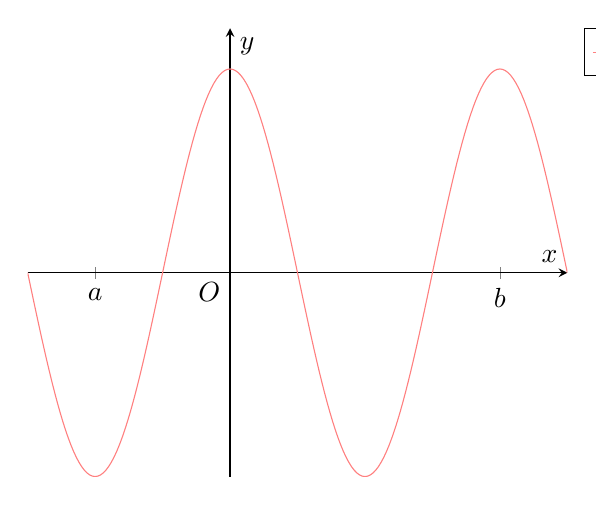
\begin{tikzpicture}[trim axis left, trim axis right]
                    \begin{axis}[
                        domain = -3*pi/2:5*pi/2,
                        samples = 201,
                        axis y line=middle,
                        axis x line=middle,
                        xlabel = {$x$},
                        ylabel = {$y$},
                        xtick={-pi, 2*pi},
                        xticklabels={$a$, $b$},
                        ytick=\empty,
                        ymax=1.2,
                        legend cell align={left},
                        legend pos=outer north east,
                        after end axis/.code={
                            \path (axis cs:0,0) 
                                node [anchor=north east] {$O$};
                            }
                        ]
                        
                        \addplot[red!50, unbounded coords=jump] {cos(\x r)};

                        \addlegendentry{$y = \cos(x)$};
                    \end{axis} 
                \end{tikzpicture}
            \end{center}

        \part
            Let $f(x) = \sec^2{x} - e^x$. Using linear interpolation on the interval $[1.5, 2.5]$,

            \begin{equation*}
                \begin{aligned}
                    a &= \dfrac{1.5f(2.5)-2.5f(1.5)}{f(2.5) - f(1.5)} \\
                    &= 1.06
                \end{aligned}
            \end{equation*}

            \boxt{
                $a = 1.06 \todp{2}$
            }

            $\sec^2{x}$ is not continuous on the interval $[1.5, 2.5]$ due to the presence of an asymptote at $x = \dfrac{\pi}2$. Hence, linear interpolation is not suitable in this case.

        \part
            We know $f^\prime(x) = 2\sec^2{x}\tan{x}-e^x$. Using the Newton-Raphson method with the initial approximation $x_1 = 0.5$,

            \begin{alignat*}{2}
                && x_1 &= 0.5 \\
                \implies&&x_2 &= \nrm{x_1}{f} = -1.02272 \\
                \implies&&x_3 &= \nrm{x_2}{f} = -0.75526 \\
                \implies&&x_4 &= \nrm{x_3}{f} = -0.40306 \\
                \implies&&x_5 &= \nrm{x_4}{f} = -0.09667 \\
                \implies&&x_6 &= \nrm{x_5}{f} = -0.00466 \\
                \implies&&x_7 &= \nrm{x_6}{f} = -0.00000
            \end{alignat*}

            As $n \rightarrow \infty$, $x_n \rightarrow 0^-$. 
            
            \begin{center}
                \begin{tikzpicture}[trim axis left, trim axis right]
                    \begin{axis}[
                        domain = -1.3:1.3,
                        samples = 201,
                        axis y line=middle,
                        axis x line=middle,
                        xlabel = {$x$},
                        ylabel = {$y$},
                        xtick={0.864, 0.5, -1.022},
                        xticklabels={$\beta$, $x_1$, $x_2$},
                        ytick=\empty,
                        ymin=-0.5,
                        ymax=1,
                        legend cell align={left},
                        legend pos=outer north east,
                        after end axis/.code={
                            \path (axis cs:0,0) 
                                node [anchor=north east] {$O$};
                            }
                        ]
                        
                        \addplot[red!50] {sec(\x r)^2 - e^x};

                        \addlegendentry{$y = \sec^2{x} - e^x$};

                        \draw[dotted] (0.5, 0) -- (0.5, -0.35);

                        \addplot[dotted, very thick] {-0.23 * (x - 0.5) - 0.35};
                    \end{axis} 
                \end{tikzpicture}
            \end{center}

            The initial approximation of $x_1 = 0.5$ is past the turning point. Hence, all subsequent approximations will converge to the root at $0$ instead of the root at $\beta$. Thus, the sequence does not converge to $\beta$.

    \problem{}
        The function $f$ is given by $f(x) = \sqrt{1 - x^2} + \cos x - 1$ for $0 \leq x \leq 1$. It is known, from graphical work, that the equation $f(x) = 0$ has a single root $x = \alpha$.

        \begin{enumerate}
            \item Express g(x) in terms of $x$, where $g(x) = x - \dfrac{f(x)}{f^\prime(x)}$.
        \end{enumerate}

        A student attempts to use the Newton-Raphson method, based on the form $x_{n+1} = g(x_n)$, to calculate the value of $\alpha$ correct to 3 decimal places.

        \begin{enumerate}
            \setcounter{enumi}{1}
            \item \begin{enumerate}
                \item The student first uses an initial approximation to $\alpha$ of $x_1 = 0$. Explain why this will be unsuccessful in finding a value for $\alpha$.
                \item The student next uses an initial approximation to $\alpha$ of $x_1 = 1$. Explain why this will also be unsuccessful in finding a value for $\alpha$.
                \item The student then uses an initial approximate to $\alpha$ of $x_1 = 0.5$. Investigate what happens in this case.
                \item By choosing a suitable value for $x_1$, use the Newton-Raphson method, based on the form $x_{n+1} = g(x_n)$, to determine $\alpha$ correct to 3 decimal places.
            \end{enumerate}
        \end{enumerate}

    \solution
        \part
            We know $f^\prime(x) = \dfrac{-x}{\sqrt{1-x^2}} - \sin x$. Hence,

            \boxt{
                $g(x) = x - \dfrac{\sqrt{1 - x^2} + \cos x - 1}{\tfrac{-x}{\sqrt{1-x^2}} - \sin x}$
            }

        \part
            \subpart
                Observe that $f^\prime(0) = 0$. Hence, $g(0)$ is undefined. Thus, starting with an initial approximation of $x_1 = 0$ will be unsuccessful in finding a value for $\alpha$.

            \subpart
                Observe that $\sqrt{1-x^2}$ is 0 when $x = 1$. Hence $f^\prime(0)$ is undefined. Thus, $g(0)$ is also undefined. Hence, starting with an initial approximation of $x_1 = 1$ will also be unsuccessful in finding a value for $\alpha$. 
            
            \subpart
                When $x_1 = 0.5$, we have $x_2 = g(x_1) = 1.20$. Since $g(x)$ is only defined for $0 \leq x \leq 1$, $x_3 = g(x_2)$ is undefined. Hence, an initial approximation of $x_1 = 0.5$ will also be unsuccessful in finding a value for $\alpha$.

            \subpart
                Using the Newton-Raphson method with $x_1 = 0.9$, we have

                \begin{alignat*}{2}
                    &&x_1 &= 0.9\\
                    \implies&&x_2 &= g(x_1) = 0.92019\\  
                    \implies&&x_3 &= g(x_2) = 0.91928\\  
                    \implies&&x_4 &= g(x_3) = 0.91928\\  
                \end{alignat*}

                \boxt{
                    $\alpha = 0.919 \todp{3}$
                }

\end{document}